\section{Architecture}
\label{sec:arch}

{\color{blue} Points to cover:

\begin{itemize}
    \item The goal: decode weak transmission by collating information from multiple base-stations
    \item Flow diagram (picture with cloudy and edgy stuff)
    \item The strawman comparison: stream everything
    \item Strawman limitations
        \begin{itemize}
            \item Weak signals and limited bandwidth (problems at gateways (could use joint decoding of preambles but cant afford to stream everything))
            \item Scaling issues (problems at the cloud)
        \end{itemize}
\end{itemize}
}


The goal of Charm is to decode weak transmission, those that could not be
decoded by any individual gateway, by collating receptions from multiple
gateways. This not only enables us to expand network coverage area but we also
describe how this saves energy on client devices.

\subsection{Energy savings on client devices}

{\color{blue} describe the power argument here...}

\begin{figure}[!htb]
\centering
\begin{tabular}{@{}c@{}}	
\subfloat[Typical client device current consumption for a complete LoRaWAN transmission. The device is powered at $3V$.]{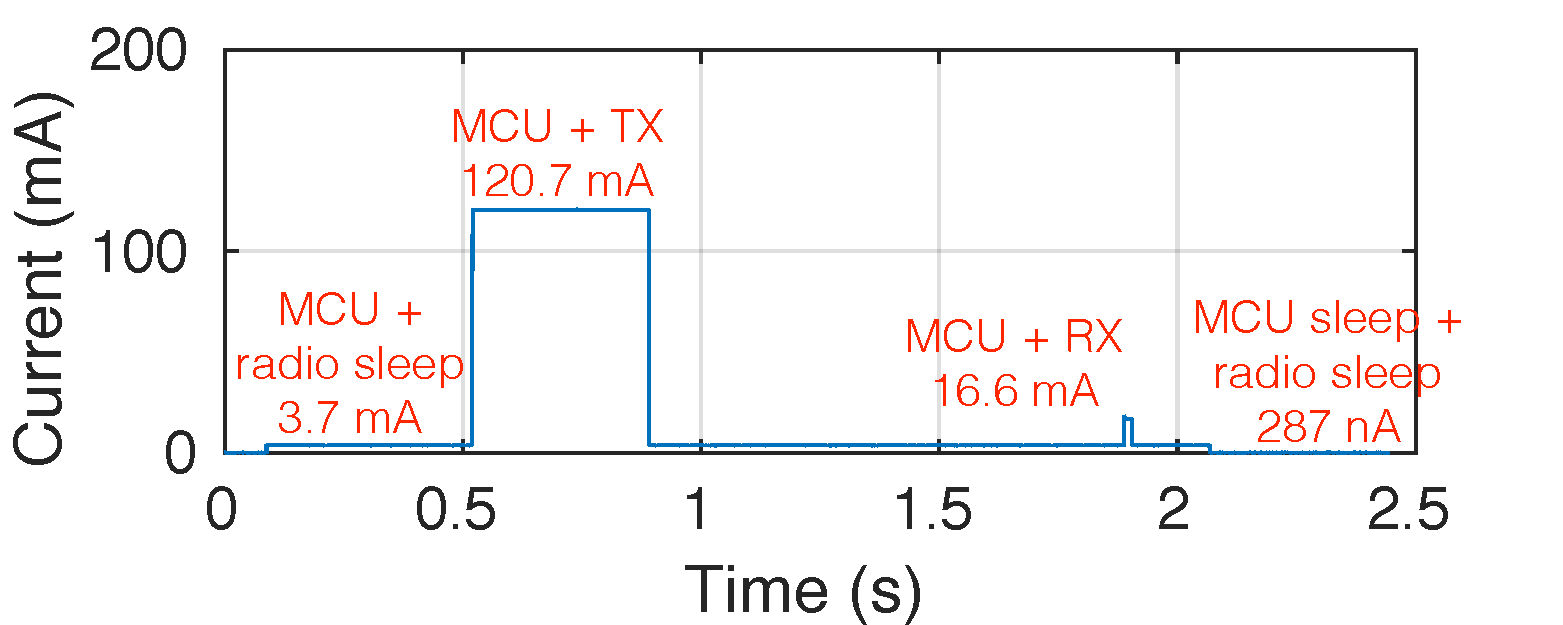
\includegraphics[width=0.4\textwidth]{figures/bug_power_trace_annotated}
\label{fig:power-trace}} \\
\subfloat[Estimated lifetime of a client device powered by two AA batteries at various bit rates based on energy profile.]{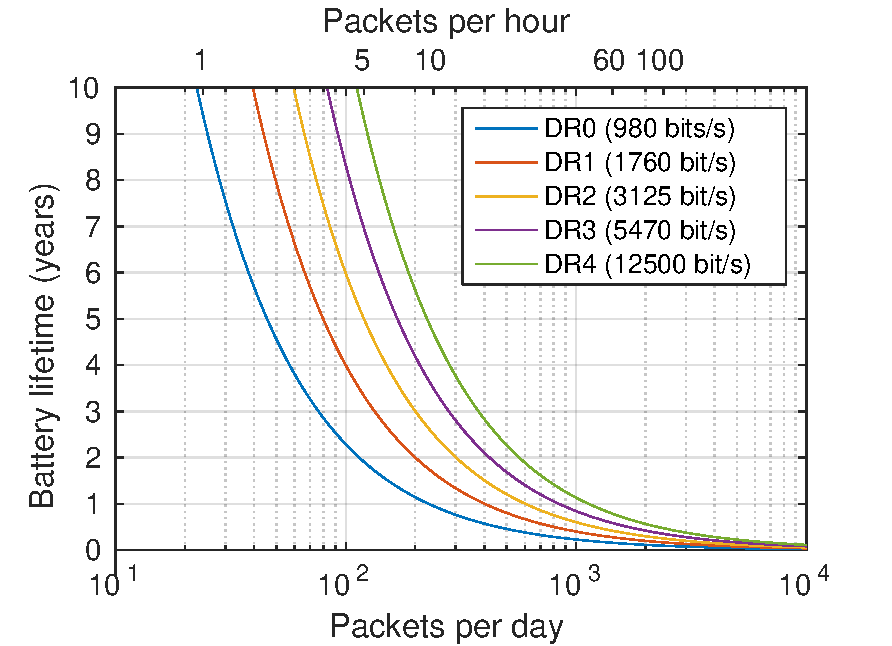
\includegraphics[width=0.4\textwidth]{figures/LoRaBug_AA_lifetime_semilog}
\label{fig:lifetime-estimates}}
\end{tabular}
\caption{}
\end{figure}

\begin{figure}[!ht]
\centering
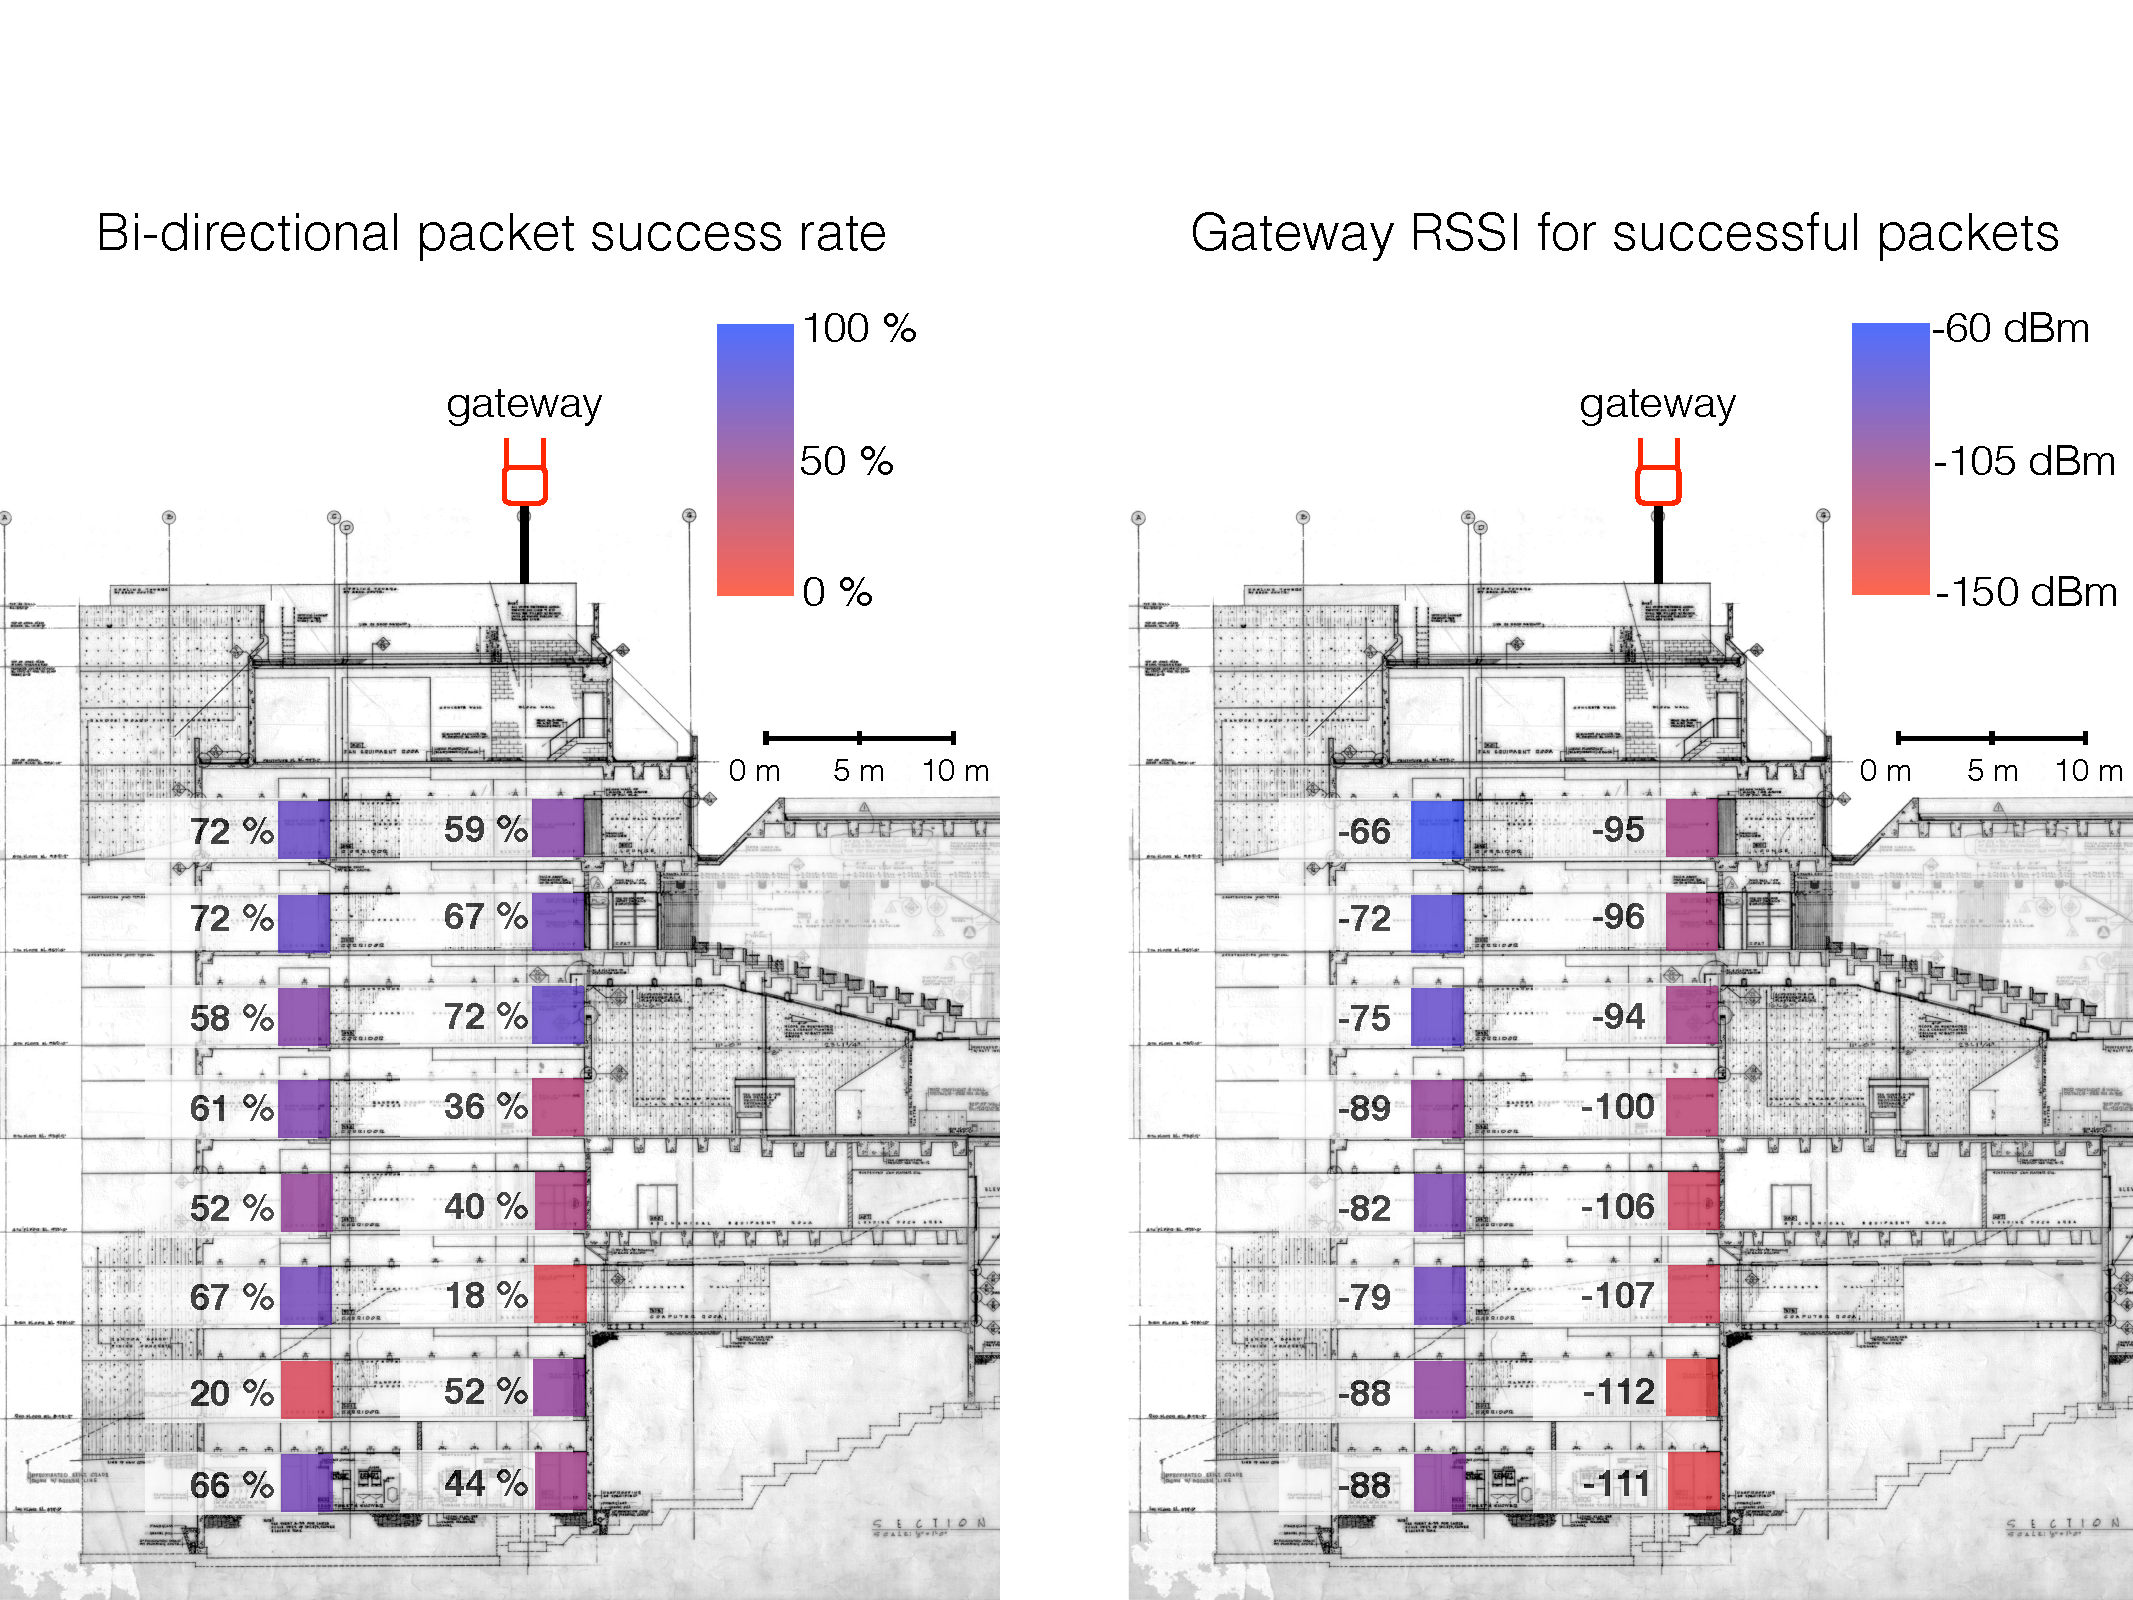
\includegraphics[width=0.5\textwidth]{figures/penetration_test_wean_cropped}
\compactimg
\caption{RF signal penetration experiments performed in a large poured-concrete building. (Left) shows the success rate for bi-directional packet exchange between end-node and gateway and (right) shows the RSSI at the gateway for successful transfers.}
\label{fig:penetration-test}
\end{figure}

Some of the transmission our system aims to decode, have signal power as low
as -30 dBm below the noise floor. Such transmission are not only impossible to
decode for an individual gateway, but they are also difficult to detect .
Since transmitted signals would combine coherently, contrasted to random noise
that combines non-coherently, an appropriate combination of radio streams
from different gateways might be able to decode such a message.

\subsection{Continuous streaming}
\label{sec:continuus-streaming}

A solution, similar to Cloud-RAN \cite{chen2011c}, is to continuously
stream all radio data to a cloud-based joint decoder. The gateways then act as
simple forwarders while all decisions and processing is done by a capable and
scaleable cloud server. This architecture is similar to LoRaWAN, but for the
physical layer. Additionally, joint detection of packets might detect even
weaker packets that what is detectable by a single receiver.

However, streaming architectures similar to Cloud-RAN suffer from two major
issues: 1. they require high bandwidth connectivity between gateways and the
cloud decoder and 2. scalability problems at the cloud with an increasing
number of gateways.

Note: continuous streaming data rate 2.250 MBps for 8 channel gateways

\subsection{Selective aggregation}
\label{sec:selective-aggregation}

{\color{blue} Describe the entire story in this section}

A: Joint decoding is good. Let's use it everywhere. Stream everything

Q: But this consumes a lot of continuous bandwidth. Most gateways will not support it. We cannot handle such a large amunt of data continuously in the cloud either.

A: LoRa packets have this nice characteristic of having a very long header. We could detect packets locally and only stream detected chunks to the cloud

Q: Our network is very vast and performance degrades near the boundaries, which also cover the most area. At any point of time there will always be many struggling transmitters.
